
\documentclass[nooutcomes]{ximera}
%\documentclass[space,handout,nooutcomes]{ximera}


% For preamble materials

\usepackage{pgf,tikz}
\usepackage{mathrsfs}
\usetikzlibrary{arrows}
\usepackage{framed}
\usepackage{amsmath}
%\pgfplotsset{compat=1.16}

\graphicspath{
  {./}
  {algorithms/}
  {../algorithms/}
}

\pdfOnly{\renewenvironment{image}[1][]{\begin{center}}{\end{center}}}

%%% This set of code is all of our user defined commands
\newcommand{\bysame}{\mbox{\rule{3em}{.4pt}}\,}
\newcommand{\N}{\mathbb N}
\newcommand{\C}{\mathbb C}
\newcommand{\W}{\mathbb W}
\newcommand{\Z}{\mathbb Z}
\newcommand{\Q}{\mathbb Q}
\newcommand{\R}{\mathbb R}
\newcommand{\A}{\mathbb A}
\newcommand{\D}{\mathcal D}
\newcommand{\F}{\mathcal F}
\newcommand{\ph}{\varphi}
\newcommand{\ep}{\varepsilon}
\newcommand{\aph}{\alpha}
\newcommand{\QM}{\begin{center}{\huge\textbf{?}}\end{center}}

\renewcommand{\le}{\leqslant}
\renewcommand{\ge}{\geqslant}
\renewcommand{\a}{\wedge}
\renewcommand{\v}{\vee}
\renewcommand{\l}{\ell}
\newcommand{\mat}{\mathsf}
\renewcommand{\vec}{\mathbf}
\renewcommand{\subset}{\subseteq}
\renewcommand{\supset}{\supseteq}
\renewcommand{\emptyset}{\varnothing}
\newcommand{\xto}{\xrightarrow}
\renewcommand{\qedsymbol}{$\blacksquare$}
\newcommand{\bibname}{References and Further Reading}
\renewcommand{\bar}{\protect\overline}
\renewcommand{\hat}{\protect\widehat}
\renewcommand{\tilde}{\widetilde}
\newcommand{\tri}{\triangle}
\newcommand{\minipad}{\vspace{1ex}}
\newcommand{\leftexp}[2]{{\vphantom{#2}}^{#1}{#2}}

%% More user defined commands
\renewcommand{\epsilon}{\varepsilon}
\renewcommand{\theta}{\vartheta} %% only for kmath
\renewcommand{\l}{\ell}
\renewcommand{\d}{\, d}
\newcommand{\ddx}{\frac{d}{dx}}
\newcommand{\dydx}{\frac{dy}{dx}}


\usepackage{bigstrut}


\newenvironment{sectionOutcomes}{}{}

\usepackage{array}
%\setlength{\extrarowheight}{-.2cm}   % Commented out by Findell to fix table headings.  Was this for typesetting division?  
\newdimen\digitwidth
\settowidth\digitwidth{9}
\def~{\hspace{\digitwidth}}
\def\divrule#1#2{
\noalign{\moveright#1\digitwidth
\vbox{\hrule width#2\digitwidth}}}



\title{Polynomials}
\author{Bart Snapp and Brad Findell and Jenny Sheldon}
\begin{document}
\begin{abstract}
Problems about polynomials.
\end{abstract}
\maketitle

\begin{problem}Explain what is meant by a \textit{polynomial} in a variable $x$.  
\begin{freeResponse}
\begin{hint}
Informally: A polynomial in $x$ is an algebraic expression that can be written as a sum of terms, each of which is a whole-number power of $x$ multiplied by some real number.  

Formally: For a whole number $n$, a \emph{polynomial (in $x$) of degree $n$} is an expression that can be written in the form 

$$a_nx^n+a_{n-1}x^{n-1}+\dots+a_1x + a_0$$

where the $a_i$'s are real numbers and $a_n\ne 0$.  
A \emph{polynomial function of degree $n$} is a function that can be defined by a polynomial.  

\end{hint}
\end{freeResponse}
\end{problem} 

%\begin{problem}
%Which of the following expressions are polynomials (select all):
%  \begin{selectAll}  
%    \choice[correct]{$x-2$}  
%    \choice{$\sqrt{x}$}
%    \choice[correct]{$1-x-x^2$}  
%    \choice{$e^x$}  
%    \choice[correct]{$56$}  
%    \choice{$\frac{2}{x}$}  
%  \end{selectAll}  
%\end{problem}

\begin{problem}
Indicate the degree of the following polynomials.  For expressions that are not polynomials, type NP.
\[
\begin{array}{cc}
 3x-3 &     \answer{1} \\
 \sqrt{x} & \answer[format=string]{NP} \\
 x^{15}  & \answer{15} \\
 1-x-x^2 & \answer{2} \\
 2^x + x^2     & \answer[format=string]{NP} \\
 (1+x)(2+x)x & \answer{3} \\
 56      & \answer{0} \\
 2/x & \answer[format=string]{NP}  
\end{array}
\]
\end{problem}

\begin{problem}Given:
\[
3x^7 -x^5 + x^4 -16x^3 + 27 = a_7 x^7 + a_6x^6 + a_5x^5 + a_4x^4 + a_3x^3 + a_2x^2 + a_1x^1 + a_0
\]
Find $a_0$, $a_1$, $a_2$, $a_3$, $a_4$, $a_5$, $a_6$, $a_7$.

Answer: $a_0=\answer{27}$, $a_1=\answer{0}$, $a_2=\answer{0}$, $a_3=\answer{-16}$, $a_4=\answer{1}$, $a_5=\answer{-1}$, $a_6=\answer{0}$, $a_7=\answer{3}$.
\end{problem} 

\begin{problem}Given:
\[
6x^5+a_4 x^4 -x^2 + a_0 = a_5 x^5 - 24 x^4 + a_3 x^3 + a_2 x^2 - 5
\]
Find $a_0$, $a_1$, $a_2$, $a_3$, $a_4$, $a_5$.

Answers: $a_0=\answer{-5}$, $a_1=\answer{0}$, $a_2=\answer{-1}$, $a_3=\answer{0}$, $a_4=\answer{-24}$, $a_5=\answer{6}$.
\end{problem} 

\begin{problem}Is it true that polynomials are equal if and only if their
  coefficients are equal? Explain your reasoning.
\begin{freeResponse}
\begin{hint}
Yes.  This is the fact we used to complete the previous two problems.
\end{hint}
\end{freeResponse}
\end{problem} 

\begin{problem}Is it true that numbers are equal if and only if their digits
  are equal? Explain your reasoning.
\begin{freeResponse}
\begin{hint}
For whole numbers written in the same base, the answer is \wordChoice{\choice[correct]{yes}\choice{no}}.  

For decimals, the answer is \wordChoice{\choice{yes}\choice[correct]{no}}.  [Note: We will learn why and how later in the course.] 

For fractions, of course, the answer is \wordChoice{\choice{yes}\choice[correct]{no}}.  For example, $\frac{2}{3}=\frac{4}{6}$, and the ``digits'' of the fraction on the left are clearly different from those of the fraction on the right. 
\end{hint}
\end{freeResponse}
\end{problem} 

\begin{problem}Explain how to add two polynomials.  Explain, in particular, how ``collecting like terms'' is
an application of the properties of arithmetic.  
\begin{freeResponse}
\begin{hint}
Use the associative and commutative properties to rearrange the sum so that like terms are consecutive.  Then use the distributive property to ``collect'' the like terms. For example, $3x^2+4x^2 = (3+4)x^2 = 7x^2$. 
\end{hint}
\end{freeResponse}
\end{problem} 

\begin{problem}Explain how to multiply two polynomials.
\begin{freeResponse}
\begin{hint}
Use the distributive property:  Multiply each term in the first polynomial by each term in the second polynomial.  Then collect like terms.  
\end{hint}
\end{freeResponse}
\end{problem} 

\begin{problem}Here is an example of the polynomial division algorithm:
\begin{image}  
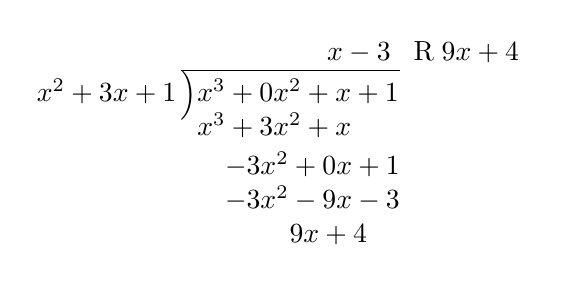
\begin{tikzpicture}  
\node at (0,0) {
$x^2 + 3x + 1\,\begin{tabular}[b]{@{}r@{}r} 
$x-3$~~&\, R\;$9x+4$\\ 
\cline{1-1}
\Big)\begin{tabular}[t]{@{}l@{}} \bigstrut[t] $x^3 + 0x^2 + x + 1$\\ 
$x^3 + 3x^2 + x$ \\ 
\divrule{0}{11}  
\bigstrut[t]~~~$-3x^2 +0x + 1$\\
~~~$-3x^2-9x -3$\\
\divrule{4}{12}
~~~~~~~~~~$9x + 4$
\end{tabular}
\end{tabular}$
};
\end{tikzpicture}
\end{image}

Describe how to perform this algorithm:  
\begin{freeResponse}
\begin{hint}
This is very much like the long division algorithm for counting numbers: 
\begin{enumerate} 
\item Write part of the quotient;
\item Multiply that part of the quotient by the divisor;
\item Subtract that product from the dividend; 
\item Repeat until the remaining part of the dividend is has a degree less than the degree of the divisor. 
\end{enumerate}
Note that, in the last step, what counts as ``less than'' is different for dividing polynomials than for dividing counting numbers.
\end{hint}
\end{freeResponse}

%\begin{enumerate}
%\item Describe how to perform this algorithm.
%\item Provide an additional relevant and revealing example
%  demonstrating that you understand the algorithm.
%\item Show the ``behind-the-scenes'' algebra that is going on here.
%\end{enumerate}\index{division algorithm!polynomial}
\end{problem} 

\begin{problem}
Find the quotient and divisor when dividing $x^3+4x^2-1$ by $x+2$.  
Quotient: $\answer{x^2+2x-4}$; remainder: $\answer{7}$. 
\end{problem}

\begin{problem}
Find the quotient and divisor when dividing $x^3+4x^2-1$ by $x^2+1$.  
Quotient: $\answer{x+4}$; remainder: $\answer{-x-5}$. 
\end{problem}


\begin{problem}State the \textit{Division Theorem} for polynomials. Give some
  relevant and revealing examples of this theorem in action.
\begin{freeResponse}
\begin{hint}
Informally, when dividing a polynomial by a (non-zero) polynomial, we can always find a sensible quotient and remainder (both polynomials).  More formally, given $n(x)$ and a non-zero divisor $d(x)$, we can find $q(x)$ and $r(x)$ such that $n(x) = \answer{d(x)q(x)+r(x)}$ with the degree of $r(x)$ \wordChoice{\choice{greater than}\choice{equal to}\choice[correct]{less than}} the degree of $d(x)$.  
\end{hint}
\end{freeResponse}
\end{problem} 



\begin{problem}
Write $35_{\text{ten}}$ in base two.
\begin{prompt}
\[
35_{\text{ten}} = \answer[given]{100011}_{\text{two}}
\]
\end{prompt}
	\begin{problem}
		Find a polynomial $p(x) = a_nx^n + a_{n-1}x^{n-1} + \dots + a_1 x + a_0$ such that the $a_i$'s are integers greater than or equal to $0$ and less than $2$ such that $p(2) = 35$.
		\begin{prompt}
			\[
			p(x) = \answer[given]{1}x^5 + \answer[given]{0}x^4 + \answer[given]{0}x^3 + \answer[given]{0}x^2 + \answer[given]{1}x + \answer[given]{1}
			\]
		\end{prompt}
		\begin{problem}
			How are the previous two problems related?
			\begin{freeResponse}
			\begin{hint}
				First, we think of our polynomial $p(x)$ as an object in base $x$.  Since the coefficients are $0$ or $1$ only, when we plug in $x=2$, we won't have to do any rearranging between the places.  So, once we plug in $x=2$, the coefficients form an element in base $x=2$.  Plugging in $x=2$ is the process we would go through to convert from base two to base ten.  So, the value of the polynomial at $x=2$ will be the base ten value of $100011_{\text{two}}$, or $35_{\text{ten}}$.
			\end{hint}
			\end{freeResponse}
		\end{problem}
	\end{problem}
\end{problem}



\begin{problem}
Consider $x^2 + 2x + 3$.  This can be thought of as a ``number'' in base $x$.  Express this number in base $x+1$, that is, find $b_0$, $b_1$, $b_2$ such that 
\[
b_2(x+1)^2 + b_1(x+1) + b_0 = x^2 + x + 1.
\]
\begin{prompt}
\[
x^2 + x + 1 = \answer[given]{1}(x+1)^2 + \answer[given]{-1}(x+1) + \answer[given]{1}.
\]
\end{prompt}
\end{problem}

\end{document}